
%(BEGIN_QUESTION)
% Copyright 2006, Tony R. Kuphaldt, released under the Creative Commons Attribution License (v 1.0)
% This means you may do almost anything with this work of mine, so long as you give me proper credit

Finn på tre ulike feil som kan forårsake at motoren på tegningen ikke starter

$$\includegraphics[width=15.5cm]{i02306x01.eps}$$

For hver av feilene, forklar \textit{hvorfor} motoren ikke vil starte. 

\underbar{file i02306}
%(END_QUESTION)





%(BEGIN_ANSWER)

Here are some possible faults (not an exhaustive list by any means!):

\begin{itemize}
\item{} Any fuse blown
\item{} Contactor coil failed open
\item{} Overload heater tripped (needs to be reset)
\item{} Any transformer winding failed open
\item{} Broken jumper between H3 and H2 on the transformer
\item{} Corroded wire connection at terminal A1 or A2
\item{} Motor winding failed shorted
\end{itemize}

\vskip 10pt

Follow-up question: there will be a difference in operation between the L1 fuse blowing and either the L2 or L3 fuse blowing.  Explain what this difference is, and why it might serve as a clue to what was wrong.

%(END_ANSWER)





%(BEGIN_NOTES)

Identifying multiple faults should be quite easy in this circuit.  The real value of this question is the opportunity for explanation and discussion that it generates for your students as they share their answers with each other.

\vskip 20pt \vbox{\hrule \hbox{\strut \vrule{} {\bf Virtual Troubleshooting} \vrule} \hrule}

This question is a good candidate for a ``Virtual Troubleshooting'' exercise.  Presenting the diagram to students, you first imagine in your own mind a particular fault in the system.  Then, you present one or more symptoms of that fault (something noticeable by an operator or other user of the system).  Students then propose various diagnostic tests to perform on this system to identify the nature and location of the fault, as though they were technicians trying to troubleshoot the problem.  Your job is to tell them what the result(s) would be for each of the proposed diagnostic tests, documenting those results where all the students can see.

During and after the exercise, it is good to ask students follow-up questions such as:

\begin{itemize}
\item{} What does the result of the last diagnostic test tell you about the fault?
\item{} Suppose the results of the last diagnostic test were different.  What then would that result tell you about the fault?
\item{} Is the last diagnostic test the best one we could do?
\item{} What would be the ideal order of tests, to diagnose the problem in as few steps as possible?
\end{itemize}

%INDEX% Electronics review: AC motor control circuit

%(END_NOTES)


